\section{离散型随机变量及其分布律}
正如微积分中,我们从数列到函数,在概率论中,我们也有一个从离散到连续的过程。有些随机变量,它的可能取值是有限个或可列无限个,这种随机变量称为\uwave{离散型随机变量}(Discrete Random Variables),相反,有些随机变量,它的可能取值是连续的,这种随机变量称为\uwave{连续型随机变量}(Continuous Random Variable)。在本节,我们先讨论较简单的离散型随机变量。

\begin{BoxDefinition}[分布律]
    设离散型随机变量$X$的可能取值以$x_k$表示,而$X$取各可能值的概率可以记为
    \begin{Equation}
        P\qty{X=x_k}=p_k\qquad k=1,2,\cdots
    \end{Equation}
    我们称上式为离散型随机变量的\uwave{分布律}(Distribution Law)。
\end{BoxDefinition}

随机变量的分布律显然应满足
\begin{Equation}
    p_k\geq 0\qquad\Sum[k=1][\infty]p_k=1
\end{Equation}

随机变量的分布律才是随机变量中我们真正关心的内容。事实上,尽管随机试验的形态很多样,但是,就其分布律而言,往往总是很有限的几种,下面我们介绍两种较典型的分布律。

\subsection{二项分布}
\begin{BoxDefinition}[伯努利试验]
    若试验$E$只有两个结果$A$和$\bar{A}$,则称$E$为\uwave{伯努利试验}(Bernoulli Experiment),记
    \begin{Equation}
        P(A)=p\qquad
        P(\bar{A})=1-p
    \end{Equation}
    将$E$独立重复进行$n$次,则称这一串重复的独立试验为$n$重伯努利试验。
\end{BoxDefinition}
这里的$n$重伯努利试验是一种很重要的数学模型,例如抛$n$次硬币($p=0.5$),例如$3$个白球和$7$个黑球的袋子中,放回抽样的摸取$n$个球($p=0.3$),其实都属于$n$重伯努利试验。

现在的问题是,$n$重伯努利试验到底会服从何种分布律呢?\goodbreak

我们以$X$表示$n$重伯努利试验中事件$A$发生的次数,这里$X$就构成了一个随机变量,我们现在来求它的分布律。很显然,这里$X$的所有可能取值为$0,1,2,\cdots,n$,由于各次试验是相互独立的,因此,事件$A$在指定的$k$次试验中发生,并且在另外$n-k$试验中不发生的概率为
\begin{Equation}
    p^k(1-p)^{n-k}
\end{Equation}
而这种指定方式,亦有$\smqty(n\\ k)$种,故事件$A$发生$k$次的概率为
\begin{Equation}
    P\qty{X=k}=\mqty(n\\ k)p^{k}(1-p)^{n-k}
\end{Equation}

这就是$n$重伯努利试验所服从的分布律,由于其类似二项式展开的形式,亦称为二项分布。
\begin{BoxDefinition}[二项分布]
    若随机变量$X$满足以下分布律
    \begin{Equation}
        P\qty{X=k}=\mqty(n\\ k)p^k(1-p)^{n-k}\qquad k=0,1,2,\cdots,n
    \end{Equation}
    则称$X$服从参数$n,p$的\uwave{二项分布}(Binomial Distribution),记为
    \begin{Equation}
        X\sim B(n,p)
    \end{Equation}
\end{BoxDefinition}
二项分布中,$k$是随机变量的取值,$n,p$则都是参量
\begin{itemize}
    \item 参量$n$代表试验的总进行次数。
    \item 参量$p$代表试验每次进行时,出现事件$A$的概率。
    \item 自变量$k$代表这$n$次试验中$A$出现的次数。
\end{itemize}

在\xref{fig:二项分布}中,我们取定$n=50$,观察$p$不同取值时二项分布$B(n,p)$随$k$的变化

\begin{Figure}[二项分布]
    \hspace{1.25cm}
    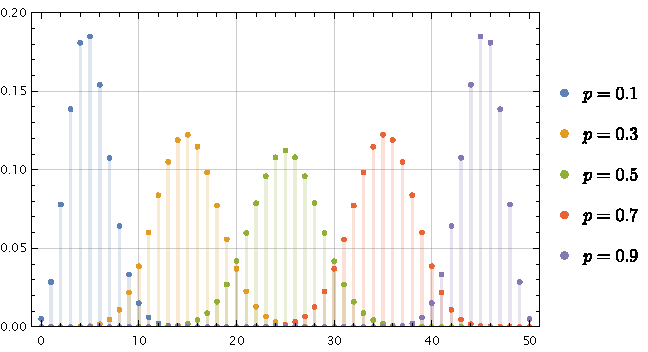
\includegraphics[scale=0.9]{Mathematica/output/BFunc.pdf}
\end{Figure}

\begin{BoxProperty}[二项分布的归一性]
    二项分布满足分布律的归一性要求
    \begin{Equation}
        \Sum[k=0][n]\mqty(n\\ k)p^k(1-p)^{n-k}=1
    \end{Equation}
\end{BoxProperty}
\begin{Proof}
    运用二项式定理可以立即得到
    \begin{Equation}*
        \Sum[k=0][n]\mqty(n\\ k)p^k(1-p)^{n-k}=[p+(1-p)]^n=1^n=1\qedhere
    \end{Equation}
\end{Proof}

特别的,对于二项分布,若取$n=1$
\begin{Equation}
    P\qty{X=k}=p^{k}\qty(1-p)^{n-k}
\end{Equation}
这相当于(一重)伯努利试验的分布律,特别的,我们称为\uwave{0--1分布}。

\subsection{泊松分布}
\begin{BoxDefinition}[泊松分布]
    若随机变量$X$满足以下分布律
    \begin{Equation}
        P\qty{X=k}=\frac{\lambda^k\e^{-\lambda}}{k!}\qquad k=0,1,2,\cdots
    \end{Equation}
    则称$X$服从参数$\lambda$的\uwave{泊松分布}(Poisson Distribution),记为
    \begin{Equation}
        X\sim P(\lambda)
    \end{Equation}
\end{BoxDefinition}

\begin{BoxProperty}[泊松分布的归一性]
    泊松分布满足分布律的归一性要求
    \begin{Equation}
        \Sum[k=0][\infty]\frac{\lambda^k\e^{-\lambda}}{k!}=1
    \end{Equation}
\end{BoxProperty}
\begin{Proof}
    运用指数函数$\e^{x}=1+x+x^2/2!+\cdots$的性质即可证明
    \begin{Equation}*
        \Sum[k=0][\infty]\frac{\lambda^k\e^{-\lambda}}{k!}=\e^{-\lambda}\Sum[k=0][\infty]\frac{\lambda^k}{k!}=\e^{-\lambda}\e^{\lambda}=1\qedhere
    \end{Equation}
\end{Proof}
泊松分布的引入与二项分布有些不同,二项分布是作为一类明确的试验模型,即$n$阶伯努利模型的分布律引入的,泊松分布则是直接给出的,这并无防碍,我们之后会逐渐了解泊松分布及其参数$\lambda$的意义。实际上,泊松分布与二项分布有密切关系,前者是后者的一种极限形式。
\begin{BoxTheorem}[泊松定理]
    设$\lambda>0$是一个常数,而$n$是任意整数,设$p_n$满足
    \begin{Equation}&[A]
        np_n=\lambda
    \end{Equation}
    则对于任何一个固定的非负整数$k$,有
    \begin{Equation}&[B]
        \Lim[n][\infty]\mqty(n\\ k)
        p_n^k(1-p_n)^{n-k}=\frac{\lambda^k\e^{-\lambda}}{k!}
    \end{Equation}
\end{BoxTheorem}
\begin{Proof}
    根据条件\xrefpeq{A},运用$p_n=\lambda/n$,并展开组合数
    \begin{Equation}&[1]
        \qquad\qquad\qquad
        \mqty(n\\ k)p_n^k(1-p_n)^{n-k}=
        \frac{n(n-1)\cdots(n-k+1)}{k!}\qty(\frac{\lambda}{n})^k\qty(1-\frac{\lambda}{n})^{n-k}
        \qquad\qquad\qquad
    \end{Equation}
    作一些调整
    \begin{Equation}&[2]
        \qquad\qquad
        \mqty(n\\ k)p_n^k(1-p_n)^{n-k}=\frac{\lambda^k}{k!}\qty[\frac{n}{n}\cdot\frac{n-1}{n}\cdots\frac{n-k+1}{n}]\qty(\frac{\lambda}{n})^k\qty(1-\frac{\lambda}{n})^{n-k}
        \qquad\qquad
    \end{Equation}
    很显然中括号内的那一项是可以化简的
    \begin{Equation}&[3]
        \qquad\qquad
        \mqty(n\\ k)p_n^k(1-p_n)^{n-k}=\frac{\lambda^k}{k!}\qty[1\cdot\qty(1-\frac{1}{n})\cdots\qty(1-\frac{k-1}{n})]\qty(\frac{\lambda}{n})^k\qty(1-\frac{\lambda}{n})^{n-k}
        \qquad\qquad
    \end{Equation}
    注意到当$n\to\infty$时
    \begin{Equation}&[4]
        \qquad
        \qty[1\cdot\qty(1-\frac{1}{n})\cdots\qty(1-\frac{k-1}{n})]\to 1\qquad
        \qty(1-\frac{\lambda}{n})^n\to \e^{-\lambda}\qquad
        \qty(1-\frac{\lambda}{n})^{-k}\to 1
        \qquad
    \end{Equation}
    因此
    \begin{Equation}*
        \Lim[n][\infty]\mqty(n\\ k)
        p_n^k(1-p_n)^{n-k}=\frac{\lambda^k\e^{-\lambda}}{k!}\qedhere
    \end{Equation}
\end{Proof}
这表明$n$很大且$p$很小的二项分布,可以近似为$\lambda=np$的泊松分布。\goodbreak

在\xref{fig:泊松分布}中,观察$\lambda$不同取值时泊松分布$P(\lambda)$随$k$的变化
\begin{Figure}[泊松分布]
    \hspace{1.25cm}
    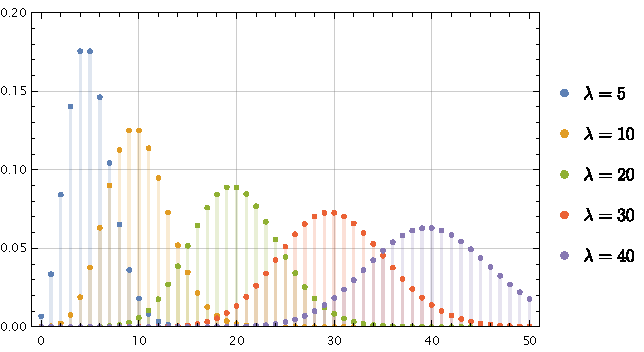
\includegraphics[scale=0.9]{Mathematica/output/PFunc.pdf}
\end{Figure}
很容易看出,参数$\lambda$越大,分布律表现的越平缓,参数$\lambda$越小,分布律越尖锐。
